\documentclass{article}

\usepackage[english]{babel}
\usepackage{listings}
\usepackage{hyperref}
\usepackage{url}
\usepackage{graphicx}
\usepackage{float}

\def\code#1{\texttt{#1}}
\def\codeblock#1{\fbox{\texttt{#1}}}

\lstset{
language=C++,
frame=single,
texcl
}

\begin{document}

\section{General IO}
\begin{itemize}
	\item \code{\#include <iostream>} IOStream package (members are in \code{namespace std})
	
	\begin{itemize}
		\item \codeblock{std::cout << output1 << output2 << ...} - Prints outputs to output stream
		
		\item \codeblock{std::cout.put(someOutput)} - Prints a single, unformatted character to output stream. \code{someOutput} is of type \code{char}.
		
		\item \codeblock{std::cin >> var} - Gets input from the input stream and stores it into var. Input is cast to type of var.
		
		\item \codeblock{char c = std::cin.get()} - Gets a single, unformatted character from the input stream.
	\end{itemize}
	
	\item \code{\#include <stdio.h>} Standard IO Library
	\begin{itemize}
		\item \codeblock{printf("myInt: \%i, myString \%s", 40, "hello")} - Prints text to the standard output stream (usually the terminal). Text is formatted according to argument 1 (a \code{const char*} type string) and arguments are specified according to in-text specifiers indicated by '\%' symbols. Any arguments specified in the format string must be added as additional arguments to the \code{printf} function. For more details, see \url{http://www.cplusplus.com/reference/cstdio/printf/}
		
		\item \codeblock{sprintf(buffer, "myInt: \%i", anotherInt)} - Formats text using the same syntax as \code{printf} but writes the completed characters into \code{buffer} (\code{buffer} is of type \code{char*})
		
		\item \codeblock{scanf("\%i", \& myInputInt)} - Reads the data from the standard input stream, formatted according to argument 1, into variable addresses specified in following arguments. For more details, see \url{http://www.cplusplus.com/reference/cstdio/scanf/}
	\end{itemize}
	
\end{itemize}

\section{Operators and Expressions}

\begin{figure}[H]
  \centering
  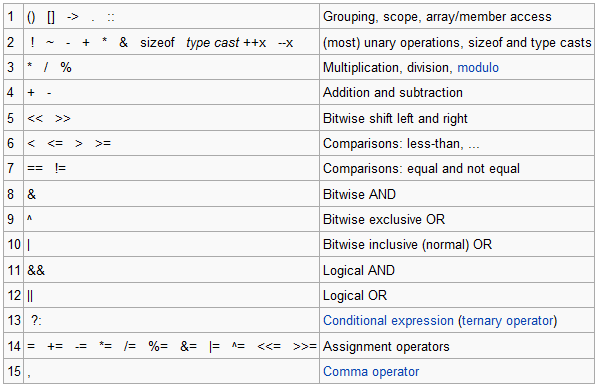
\includegraphics[width=1\textwidth]{SRC/order-of-ops}
  \caption{Order of Operations in C++}
\end{figure}

\subsection{Bitwise Operators}

\begin{lstlisting}
unsigned char X = 55; // 00110111
unsigned char Y = 15; // 00001111
\end{lstlisting}

\begin{itemize}
	\item \codeblock{unsigned char Z = X \& Y} - Logical AND between X and Y. Z is now 00000111
	\item \codeblock{unsigned char Z = X | Y} - Logical OR between X and Y. Z is now 00111111
	\item \codeblock{unsigned char Z = Y \^ Y} - Logical XOR between X and Y. Z is now 00111000
	\item \codeblock{unsigned char Z = X >> 1} - Bit shift in the direction of the LSB. Z is now 00011011
	\item \codeblock{unsigned char Z = X << 1} - Bit shift in the direction of the MSB. Z is now 01101110
	\item \codeblock{unsigned char Z = ~X;} - Logical NOT. Z is now 11001000
\end{itemize}

\section{Control and Loop Structures}

\subsection{If-Then-Else}
\begin{lstlisting}
if (<Some logical expression>) {
	// Do some stuff
}
else if (<Some other expression>) // Do other stuff;
else {
	// more stuff here
}
\end{lstlisting}

\subsection{Switch}
\begin{lstlisting}
switch(<some value>) {
	case 0:
		\\ Case 1
		break;
	case 1:
	case 2:
		\\ This executes for cases 1 and 2!
		break;
	default:
		\\ Do this if all else fails
}
\end{lstlisting}
\emph{Note:} great for when there are a bunch of known possible values. Essentially shorthand for a long if-then-else statement

\subsection{Ternary Statement}
\begin{lstlisting}
X = <expression> ? <return if true> : <return if false>
\end{lstlisting}
\emph{Note:} great for simple if else statements like when toggling a variable between two values

\subsection{While Loop}
\begin{lstlisting}
int X = 0;
while (X < 10) {
	// Do some stuffs
	X++;
}
\end{lstlisting}

\subsection{For Loop}
\begin{lstlisting}
for (int X = 0; X < 10; X++) {
	// Do some stuffs
}
\end{lstlisting}

\section{Functions}

\subsection{Arguments by Value}
\begin{lstlisting}
int add(int arg1, int arg2) {
	return arg1 + arg2;
}

int X = 10;
int Y = 10;
int Z = add(X, Y);
\end{lstlisting}

\subsection{Arguments by Pointer Value}
\begin{lstlisting}
void add(int* arg1, int* arg2, int* sum) {
	*sum = *arg1 + *arg2;
}

int X = 10;
int Y = 10;
int Z = 0;
add(&X, &Y, &Z);
\end{lstlisting}
\emph{Note:} passing arguments by pointer value (address) only has to transfer the size of the pointer itself (usually 4-8 bytes depending on the machine). This can be dramatically faster when passing in large arrays of values such as strings or number lists. 

\subsection{Arguments by Reference}
\begin{lstlisting}
void add(int& arg1, int& arg2, int& sum) {
	sum = arg1 + arg2;
}

int X = 10;
int Y = 10;
int Z = 0;
add(X, Y, Z);
\end{lstlisting}

\emph{Note:} passing by reference is only shorthand for passing arguments by pointer value (address). However, it can be confusing to work with since the syntax are nearly the same as passing by value so don't use them unless you know what you're doing.
	
\end{document}